% !TEX encoding = UTF-8 Unicode
% !TEX program = xelatex

\documentclass{article}
	\usepackage{fontspec}
	\usepackage{tikz}
	\usepackage{listings}
\begin{document}



	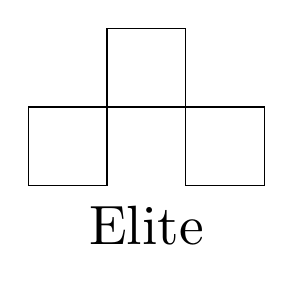
\begin{tikzpicture}
		\draw (0, 0) rectangle (1, 1);
		\draw [shift = {(1, 1)}] (0, 0) rectangle (1, 1);
		\draw [shift = {(2, 0)}] (0, 0) rectangle (1, 1);
		\node at (1.5, -0.5) [scale = 2] {Elite};
	\end{tikzpicture}




\fontspec{SourceCodePro-Regular}
\lstset{
	language=[latex]tex,tabsize=4,
	moredelim=*[s][\itshape]{$}{$},
	moredelim=*[s][\color{red!40!.}]{(}{)},
	moredelim=*[s][\color{green!30!.}]{[}{]},
	backgroundcolor=\color{blue!5},
	commentstyle=\color{.!80}\itshape,
	texcsstyle=*\color{blue!40!.},
	moretexcs={
		node,
	},
	deletetexcs={},
}
\lstinputlisting{transform.tex}

\end{document}